% =============================================================================
%  Introducción a la Optimización Numérica
%  Diapositivas en español basadas en:
%    S. L. Brunton, "Optimization: A Bootcamp for Machine Learning,
%    Inverse Problems, and Control", Cambridge University Press, 2025.
%    Capítulo 1, secciones 1.1--1.5.
%
%  Compilar con:  pdflatex intro_OptimizacionNumerica.tex  (varias veces)
%  o bien:        make
% =============================================================================

\documentclass[10pt,aspectratio=169]{beamer}

% --- Idioma y codificación ---------------------------------------------------
\usepackage[utf8]{inputenc}
\usepackage[T1]{fontenc}
\usepackage[spanish]{babel}

% --- Matemáticas -------------------------------------------------------------
\usepackage{amsmath,amssymb,amsthm,mathtools}
\usepackage{lmodern}
\usepackage{microtype}

% --- Gráficos y figuras ------------------------------------------------------
\usepackage{graphicx}
\usepackage{tikz}
\usetikzlibrary{calc}

% --- Teoremas ----------------------------------------------------------------
\theoremstyle{definition}
\newtheorem{definicion}{Definición}
\newtheorem{ejemplo}{Ejemplo}

\theoremstyle{plain}
\newtheorem{teorema}{Teorema}
\newtheorem{lema}{Lema}
\newtheorem{corolario}{Corolario}
\newtheorem{prop}{Proposición}

\setbeamertemplate{navigation symbols}{}
\setbeamertemplate{footline}[frame number]

% --- Metadatos ---------------------------------------------------------------
\title{Introducción a la\\Optimización Numérica}
\subtitle{Conceptos fundamentales: anatomía, convexidad,\\
          gradientes, restricciones y aplicaciones}
\institute{Maestría en Matemática --- UNAH\\
           Universidad Nacional Autónoma de Honduras}
\date{\today}

% Helper: empty figure placeholder that reserves a fixed bottom slot.
% Use: \figura{Etiq. del contenido pendiente}{0.78\textwidth}{1.6cm}
\newcommand{\figura}[3]{%
  \vfill
  \begin{center}
    \fbox{\parbox[c][#3][c]{#2}{\centering
      \textit{[figura pendiente]}\par\medskip
      \scriptsize\textbf{Contenido:} \textit{#1}%
    }}%
  \end{center}%
}

% =============================================================================
\begin{document}
% =============================================================================

% --- Portada -----------------------------------------------------------------
\begin{frame}
  \titlepage
\end{frame}

% --- Resumen / esquema -------------------------------------------------------
\begin{frame}{Esquema de la presentación}
  \tableofcontents
\end{frame}

% =============================================================================
\section{Anatomía de un problema de optimización}
% =============================================================================

\begin{frame}[t]{Forma estándar de un problema de optimización}
  \begin{block}{Problema sin restricciones}
    En su forma más simple, optimizamos una \emph{función objetivo}
    $f:\mathbb{R}^{n}\to\mathbb{R}$ sobre una \emph{variable de decisión}
    $x\in\mathbb{R}^{n}$:
    \[
      \min_{x\in\mathbb{R}^{n}} f(x).
    \]
    En una variable basta con buscar $x$ donde $f'(x)=0$ y $f''(x)>0$.
  \end{block}

  \vspace{0.15em}
  \begin{block}{Forma estándar con restricciones (Ec.~(1.2)--(1.3))}
    \begin{align*}
      \min_{x}\;     & f(x) \\
      \text{s.a. }   & g_{i}(x) \leq 0,\;\; i=1,\dots,m,\\
                     & h_{j}(x) = 0,\;\; j=1,\dots,p.
    \end{align*}
    Las restricciones definen el \emph{conjunto factible}
    $\mathcal{S}=\{x : g(x)\leq 0,\; h(x)=0\}$.
  \end{block}

  \vspace{0.2em}
  \begin{itemize}\setlength\itemsep{0pt}
    \item Maximizar una $f$ cóncava equivale a minimizar $-f$ (convexa).
    \item En un programa lineal $f(x)=c^{\top}x$ es convexa \emph{y} cóncava.
  \end{itemize}
\end{frame}

\begin{frame}[t]{Anatomía visual y ejemplo introductorio}
  \begin{ejemplo}[Panel 1.1: proyectil]
    El alcance de un proyectil lanzado con rapidez $v$ a ángulo $\alpha$ es
    \[
      D(\alpha) \;=\; \frac{v^{2}}{g}\,\operatorname{sen}(2\alpha).
    \]
    Derivando: $D'(\alpha)=0$ en el óptimo $\Rightarrow \alpha^{*}=\pi/4$.
    \emph{El óptimo sin restricción está en el borde del dominio factible.}
  \end{ejemplo}

  \vspace{0.2em}
  \textbf{Ingredientes del problema:}
  \begin{itemize}\setlength\itemsep{0pt}
    \item \emph{Función objetivo} $f(x)$.
    \item \emph{Variable de decisión} $x\in\mathbb{R}^{n}$.
    \item \emph{Restricciones} de igualdad $h$ y desigualdad $g$.
    \item \emph{Conjunto factible} $\mathcal{S}=\{x:g\leq 0,\,h=0\}$.
  \end{itemize}
  \begin{figure}
      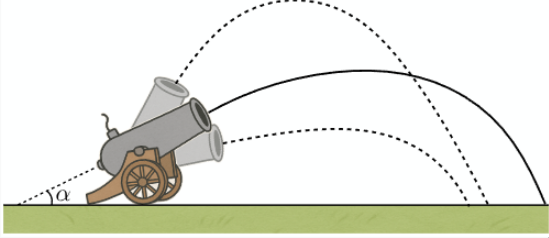
\includegraphics[width=0.3\textwidth]{images/canon.png}
  \end{figure}

\end{frame}

\begin{frame}[t]{Problemas comunes: LP y QP}{Ejemplos clave en la práctica}
  \begin{columns}[T]
    \column{0.48\textwidth}
    \begin{block}{Programación lineal (LP)}
      \begin{align*}
        \max_{x}\;     & c^{\top} x \\
        \text{s.a. } & Ax \leq b,\quad x\geq 0.
      \end{align*}
      Objetivo y restricciones son lineales; el conjunto factible
      $\mathcal{S}$ es un \emph{politopo}.
      \emph{El óptimo está en un vértice del politopo.}
    \end{block}

    \column{0.48\textwidth}
    \begin{block}{Programación cuadrática (QP)}
      \begin{align*}
        \min_{x}\;     & \tfrac{1}{2}\,x^{\top} Q x + c^{\top} x \\
        \text{s.a. } & Ax \leq b,\quad x\geq 0.
      \end{align*}
      \emph{Convexa} si $Q\succeq 0$ (semidefinida positiva).
      Ejemplo central: \emph{mínimos cuadrados}
      $\min_{x}\tfrac{1}{2}\|Ax-b\|_{2}^{2}$, con $Q=A^{\top}A$.
    \end{block}
  \end{columns}

  \begin{figure}
      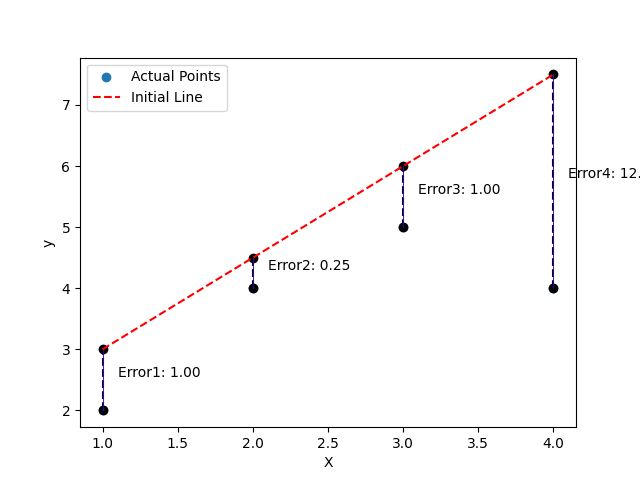
\includegraphics[width=0.3\textwidth]{images/least_squares.png}
  \end{figure}

\end{frame}

\begin{frame}[t]{Preguntas frecuentes sobre la función objetivo}
  Antes de elegir un algoritmo, conviene hacerse estas preguntas sobre $f$:

  \begin{block}{¿$f$ es convexa?}
    Si $f$ y $\mathcal{S}$ son convexos, \emph{todo óptimo local es global}.
    Mínimos cuadrados lineales es convexo; entrenar una red neuronal, no.
  \end{block}

  \begin{block}{¿Podemos calcular $\nabla f$?}
    Si sí: descenso por gradiente o Newton (Cap.~2).
    Si no: métodos sin gradiente (Cap.~5) o adjunto / surrogate.
  \end{block}

  \begin{block}{¿$f$ es lineal, cuadrática, general?}
    Lineal $\Rightarrow$ LP. Cuadrática con Hessiana $H\succ 0 \Rightarrow$ convexa;
    $H$ indefinida $\Rightarrow$ punto silla; $H$ negativa $\Rightarrow$ cóncava.
  \end{block}

  \begin{block}{Otras preguntas}
    ¿Alta dimensión? ¿$f$ desconocida / caja negra? ¿Cara de evaluar?
    ¿Codifica dinámica temporal? Cada pregunta cambia el método apropiado.
  \end{block}
\end{frame}

% =============================================================================
\section{Convexidad en optimización}
% =============================================================================

\begin{frame}[t]{Conjuntos convexos}
  \begin{definicion}[Conjunto convexo]
    Un conjunto $C\subseteq\mathbb{R}^{n}$ es \emph{convexo} si para todo
    par $x,y\in C$ y todo $\alpha\in[0,1]$:
    \[
      \alpha x + (1-\alpha)y \;\in\; C.
    \]
    Geométricamente: \emph{el segmento que une dos puntos de $C$ está
    completamente contenido en $C$}.
  \end{definicion}

  \vspace{0.2em}
  \begin{teorema}[Intersección de convexos]
    Si $C_{1},C_{2}\subseteq\mathbb{R}^{n}$ son convexos, entonces
    $C = C_{1}\cap C_{2}$ también es convexo.
  \end{teorema}

  \begin{proof}
    Sean $x,y\in C$. Entonces $x,y\in C_{1}$ y $x,y\in C_{2}$.
    Por convexidad de $C_{1}$, $\alpha x+(1-\alpha)y\in C_{1}$ para todo
    $\alpha\in[0,1]$. Lo mismo para $C_{2}$. Luego
    $\alpha x+(1-\alpha)y\in C_{1}\cap C_{2}=C$.
  \end{proof}

  \vspace{0.2em}
  \textbf{Ejemplos:} puntos, líneas, planos, semiespacios, bolas
  $B_{r}=\{x:\|x\|_{2}\leq r\}$, elipsoides rellenos, conos convexos.
  \emph{Politopos} $\mathcal{S}=\{x:Ax\leq b\}$ son convexos.

  \url{https://en.wikipedia.org/wiki/Convex_set}
\end{frame}

\begin{frame}[t]{Funciones convexas y normas}
  \begin{definicion}[Función convexa]
    $f:\mathbb{R}^{n}\to\mathbb{R}$ es \emph{convexa} si para todo
    $x,y$ y $\alpha\in[0,1]$:
    \[
      f\bigl(\alpha x+(1-\alpha)y\bigr) \;\leq\;
      \alpha f(x)+(1-\alpha)f(y).
    \]
    \emph{Convexidad estricta} si la desigualdad es estricta para $x\neq y$.
  \end{definicion}

  \vspace{0.2em}
  \begin{prop}[Normas son convexas]
    Toda norma $\|\cdot\|$ es convexa: usando la desigualdad triangular,
    \begin{align*}
      \|\alpha x + (1-\alpha)y\|
      &\leq \|\alpha x\| + \|(1-\alpha)y\| \\
      &= \alpha\|x\| + (1-\alpha)\|y\|.
    \end{align*}
  \end{prop}

  \vspace{0.2em}
  \textbf{Otras propiedades:} $f+g$ convexas $\Rightarrow f+g$ convexa.
  $f$ convexa $\Rightarrow -f$ cóncava. Composición afín $f(Ax+b)$ conserva
  convexidad. $\mathrm{epi}(f)=\{(x,y):y\geq f(x)\}$ es convexo
  $\Leftrightarrow$ $f$ es convexa.
  \url{https://en.wikipedia.org/wiki/Convex_function}

\end{frame}

\begin{frame}[t]{El teorema central de la optimización convexa}
  \begin{teorema}[Óptimo local = óptimo global]
    Sea $f$ una función convexa sobre un conjunto convexo $\mathcal{S}$.
    Entonces todo \emph{mínimo local} de $f$ sobre $\mathcal{S}$ es también
    un \emph{mínimo global}. Si $f$ es estrictamente convexa, el mínimo
    es único.
  \end{teorema}

  \begin{proof}[Prueba por contradicción]
    Supongamos que $x$ es mínimo local en $\mathcal{S}$, así que existe
    $\epsilon>0$ tal que $f(z)\geq f(x)$ para todo $z\in\mathcal{S}\cap B_{\epsilon}(x)$.
    Supongamos además que existe $y\in\mathcal{S}$ con $f(y)<f(x)$.

    Como $\mathcal{S}$ es convexo, todo punto del segmento
    $\{z=(1-\alpha)x+\alpha y:\alpha\in[0,1]\}$ es factible. Eligiendo
    $\alpha_{1}=\epsilon/\|y-x\|_{2}$ y $\alpha_{2}=\alpha_{1}/2$, el punto
    $z=(1-\alpha_{2})x+\alpha_{2}y$ cae dentro de la $\epsilon$-bola.
    Por convexidad y dado que $f(y)<f(x)$:
    \[
      f(z) \;\leq\; \alpha_{2}f(y)+(1-\alpha_{2})f(x) \;<\; f(x),
    \]
    contradiciendo que $x$ fuese mínimo local.
  \end{proof}

  \vspace{0.15em}
  \begin{corolario}
    En LP y en mínimos cuadrados lineales \emph{todo óptimo local es global}.
  \end{corolario}
\end{frame}

\begin{frame}[t]{La desigualdad de Jensen}
  \begin{teorema}[Desigualdad de Jensen]
    Sean $x_{1},\dots,x_{m}\in\mathbb{R}^{n}$ y $\alpha_{1},\dots,\alpha_{m}\geq 0$
    con $\sum_{k=1}^{m}\alpha_{k}=1$. Para toda $f$ convexa:
    \[
      f\!\left(\sum_{k=1}^{m}\alpha_{k}x_{k}\right)
      \;\leq\; \sum_{k=1}^{m}\alpha_{k}f(x_{k}).
    \]
  \end{teorema}

  \vspace{0.2em}
  \begin{ejemplo}[Aplicación probabilística]
    Con $p(x)\geq 0$, $\int p(x)\,dx=1$, la generalización a integrales da
    \[
      f\bigl(\mathbb{E}[x]\bigr) \;\leq\; \mathbb{E}\bigl[f(x)\bigr].
    \]
    En particular $(\mathbb{E}[x])^{2}\leq\mathbb{E}[x^{2}]$ (tomando $f(t)=t^{2}$).
  \end{ejemplo}

  \figura{Interpretación geométrica: cualquier politopo formado por $m$ puntos
          sobre la función está enteramente contenido en el epígrafe.}
          {0.78\textwidth}{1.6cm}
\end{frame}

% =============================================================================
\section{Gradientes y la geometría de la optimización}
% =============================================================================

\begin{frame}[t]{El gradiente: definición}
  \begin{definicion}[Gradiente]
    Para $f:\mathbb{R}^{n}\to\mathbb{R}$, el \emph{gradiente} es
    \[
      \nabla f(x) \;=\;
      \begin{bmatrix}\partial f/\partial x_{1}\\ \vdots \\ \partial f/\partial x_{n}\end{bmatrix}
      \;\in\;\mathbb{R}^{n}.
    \]
    Cada componente $\partial f/\partial x_{k}$ mide cuánto cambia $f$ al
    variar $x_{k}$.
  \end{definicion}

  \vspace{0.15em}
  \textbf{Aproximación de primer orden (Ec.~(1.24)):}
  \[
    f(x) \;\approx\; f(x_{0}) + \nabla f(x_{0})^{\top}(x-x_{0}).
  \]
  Así, $\nabla f(x_{0})^{\top}\Delta x$ aproxima el cambio de $f$ ante un
  desplazamiento pequeño $\Delta x = x-x_{0}$.

  \figura{El gradiente define el plano tangente en $x_{0}$. (Brunton, Fig.~1.19.)}
          {0.78\textwidth}{1.6cm}
\end{frame}

\begin{frame}[t]{El gradiente: interpretación geométrica}
  \begin{prop}[Dirección de máximo crecimiento]
    El producto interior $\nabla f(x_{0})^{\top}\Delta x$ se maximiza cuando
    $\Delta x$ es paralelo a $\nabla f(x_{0})$. Por tanto:
    \begin{itemize}\setlength\itemsep{0pt}
      \item $+\nabla f(x_{0})$: dirección de \emph{máximo crecimiento}.
      \item $-\nabla f(x_{0})$: dirección de \emph{máximo descenso local},
            base del descenso por gradiente (Cap.~2).
    \end{itemize}
  \end{prop}

  \vspace{0.15em}
  \textbf{Tangente y plano tangente:} $\nabla f(x_{0})$ generaliza la
  derivada escalar $f'(x_{0})$ al caso vectorial: la derivada define la recta
  tangente en una variable; el gradiente define el \emph{plano (o
  hiperplano) tangente} en varias.

  \vspace{0.15em}
  \begin{lema}[Soporte desde abajo]
    Para $f$ diferenciable y convexa, el plano tangente en $x_{0}$ acota
    $f$ desde abajo:
    \[
      f(x) \;\geq\; f(x_{0}) + \nabla f(x_{0})^{\top}(x-x_{0})
      \qquad \forall\,x.
    \]
    \emph{Si existe $x^{*}$ con $\nabla f(x^{*})=0$, entonces $x^{*}$ es
    mínimo global.}
  \end{lema}
\end{frame}

\begin{frame}[t]{Hessiana y convexidad de segundo orden}
  \begin{definicion}[Matriz Hessiana]
    Para $f$ dos veces continuamente diferenciable, la \emph{Hessiana} es
    \[
      H(x) \;=\; \nabla^{2} f(x) \;=\;
      \begin{bmatrix}
        \partial^{2}f/\partial x_{1}^{2} & \cdots & \partial^{2}f/\partial x_{1}\partial x_{n}\\
        \vdots & \ddots & \vdots\\
        \partial^{2}f/\partial x_{n}\partial x_{1} & \cdots & \partial^{2}f/\partial x_{n}^{2}
      \end{bmatrix}.
    \]
  \end{definicion}

  \vspace{0.2em}
  \begin{teorema}[Condición de segundo orden para convexidad]
    Una $f\in C^{2}$ es convexa si y sólo si $H(x)=\nabla^{2}f(x)\succeq 0$
    (semidefinida positiva) para todo $x$. Si $H(x)\succ 0$, $f$ es
    \emph{estrictamente} convexa.
  \end{teorema}

  \begin{proof}[Idea]
    Expansión de Taylor de segundo orden:
    \[
      f(x) \;\approx\; f(x_{0}) + \nabla f(x_{0})^{\top}(x-x_{0})
                + \tfrac{1}{2}(x-x_{0})^{\top}\nabla^{2}f(x_{0})(x-x_{0}).
    \]
    El término cuadrático es no negativo si y sólo si $H\succeq 0$.
  \end{proof}

  \vspace{0.2em}
  \begin{ejemplo}[Ajuste lineal]
    $f(a,b)=\sum_{j}(ax_{j}+b-y_{j})^{2}$. Imponiendo $\nabla f=0$ se obtienen
    las \emph{ecuaciones normales}
    $\begin{bmatrix}\sum x_{j}^{2} & \sum x_{j}\\ \sum x_{j} & n\end{bmatrix}
      \begin{bmatrix}a\\ b\end{bmatrix}
      = \begin{bmatrix}\sum x_{j}y_{j}\\ \sum y_{j}\end{bmatrix}$.
  \end{ejemplo}
\end{frame}

% =============================================================================
\section{Restricciones y multiplicadores de Lagrange}
% =============================================================================

\begin{frame}[t]{Restricciones de igualdad: el Lagrangiano}
  \begin{block}{Problema con restricciones de igualdad}
    \begin{align*}
      \min_{x}\;     & f(x) \\
      \text{s.a. } & h(x)=0.
    \end{align*}
  \end{block}

  \vspace{0.15em}
  Idea clave: añadir una \emph{penalización}
  $\delta_{0}(h(x))$ (vale $0$ si $h(x)=0$, $+\infty$ en otro caso) y suavizarla como $\lambda h(x)$:
  \[
    \min_{x}\max_{\lambda}\; \underbrace{f(x)+\lambda h(x)}_{L(x,\lambda)}.
    \tag{Ec.~(1.30)}
  \]
  A $L(x,\lambda)$ se le llama \emph{Lagrangiano} y a $\lambda$ el
  \emph{multiplicador de Lagrange}.

  \vspace{0.2em}
  El \emph{problema dual} (Ec.~(1.31)) se obtiene intercambiando el orden
  $\min$ y $\max$: $\max_{\lambda}\min_{x}L(x,\lambda)$.

  \figura{Plano tangente al conjunto factible en el óptimo. (Brunton, Fig.~1.21.)}
          {0.78\textwidth}{1.6cm}
\end{frame}

\begin{frame}[t]{Condición de optimalidad y ejemplos}
  \begin{teorema}[Condición necesaria de primer orden]
    Si $x^{*}$ resuelve el problema con restricción $h(x^{*})=0$ y
    $\nabla h(x^{*})\neq 0$ (cualificación de regularidad), entonces existe
    $\lambda^{*}\in\mathbb{R}$ tal que
    \begin{align*}
      \nabla_{x} L(x^{*},\lambda^{*}) &= \nabla f(x^{*}) + \lambda^{*}\nabla h(x^{*}) = 0,\\
      \nabla_{\lambda} L(x^{*},\lambda^{*}) &= h(x^{*}) = 0.
    \end{align*}
    \emph{Los gradientes de la objetivo y de la restricción activa son
    paralelos en el óptimo.}
  \end{teorema}

  \vspace{0.2em}
  \begin{ejemplo}[Restricción activa]
    $\min\,(x-1)^{2}+1$ s.a.\ $x\leq 0$.
    El óptimo sin restricción es $x^{*}=1$, pero la restricción lo empuja
    al borde: $x^{*}=0$, $\lambda^{*}=2$.
    Verificación: $\nabla f(x^{*})=-2$, $\nabla g(x^{*})=1$, luego
    $\nabla f+\lambda\nabla g=0 \Leftrightarrow \lambda^{*}=2$.
  \end{ejemplo}

  \vspace{0.2em}
  \begin{ejemplo}[Restricción inactiva]
    Misma formulación con $f(x)=(x+1)^{2}+1$. El óptimo $x^{*}=-1$ ya
    satisface $g(x^{*})<0$, así que la restricción es inactiva y
    $\lambda^{*}=0$.
  \end{ejemplo}
\end{frame}

\begin{frame}[t]{KKT para restricciones mixtas}
  \begin{block}{Problema general con restricciones mixtas}
    \begin{align*}
      \min_{x}\;     & f(x) \\
      \text{s.a. } & g_{i}(x)\leq 0,\;\; i=1,\dots,m,\\
                   & h_{j}(x)=0,\;\; j=1,\dots,p.
    \end{align*}
    El Lagrangiano es
    $L(x,\lambda,\mu)=f(x)+\sum_{i}\lambda_{i}g_{i}(x)+\sum_{j}\mu_{j}h_{j}(x)$.
  \end{block}

  \vspace{0.2em}
  \begin{teorema}[Condiciones KKT (Karush--Kuhn--Tucker)]
    Bajo cualificaciones de regularidad (p.ej.\ Slater), existe
    $(\lambda^{*},\mu^{*})$ con
    \begin{align*}
      \nabla f(x^{*}) + \textstyle\sum_{i}\lambda_{i}^{*}\nabla g_{i}(x^{*})
                                   + \sum_{j}\mu_{j}^{*}\nabla h_{j}(x^{*}) &= 0,\\
      g_{i}(x^{*}) \leq 0,\quad h_{j}(x^{*}) &= 0,\\
      \lambda_{i}^{*}\geq 0,\quad \lambda_{i}^{*}g_{i}(x^{*}) &= 0
      \qquad\text{(complementariedad)}.
    \end{align*}
    La \emph{complementariedad} fuerza $\lambda_{i}^{*}=0$ si la restricción
    es \emph{inactiva} ($g_{i}(x^{*})<0$).
  \end{teorema}

  \vspace{0.2em}
  La formulación de Slater y el análisis riguroso de estas condiciones se
  desarrollan en el Cap.~6 del texto guía.
\end{frame}

% =============================================================================
\section{Aplicaciones de la optimización}
% =============================================================================

\begin{frame}[t]{Problemas inversos}
  \begin{block}{Formulación general}
    Dado un \emph{modelo directo} $F$ y observaciones $y_{\text{obs}}$,
    buscamos parámetros $x$ tales que $F(x)\approx y_{\text{obs}}$, es decir,
    \[
      \min_{x}\; \|F(x) - y_{\text{obs}}\|_{2}^{2}.
    \]
  \end{block}

  \vspace{0.2em}
  Los datos son típicamente \emph{parciales y ruidosos}, así que el problema
  suele ser \emph{mal planteado} o \emph{mal condicionado}. Las soluciones
  estándar combinan:
  \begin{itemize}\setlength\itemsep{0pt}
    \item \emph{Regularización}: añadir $\|x\|^{2}$, $\|x\|_{1}$, etc.
    \item \emph{Relajación}: sustituir normas no convexas ($\ell_{0}$) por
          convexas ($\ell_{1}$, nuclear).
    \item \emph{Priors bayesianos} (Cap.~7).
  \end{itemize}

  \vspace{0.15em}
  \textbf{Aplicaciones:} tomografía computarizada (CT), resonancia magnética
  (MRI), super-resolución, inversión sísmica, identificación de sistemas,
  diseño de perfiles aerodinámicos.

  \figura{Esquema de un problema inverso: ajustar $x$ para que $F(x)$
          coincida con los datos observados.}
          {0.78\textwidth}{1.6cm}
\end{frame}

\begin{frame}[t]{Teoría de control}
  \begin{block}{Lazo cerrado}
    La señal del sensor $y$ se compara con la referencia $r$; el error
    $\varepsilon=r-y$ alimenta al controlador, que produce la acción
    $u=k(x)$ sobre la planta:
    \begin{equation*}
      \dot{x} \;=\; f(x,u), \qquad u \;=\; k(x).
    \end{equation*}
  \end{block}

  \vspace{0.2em}
  El objetivo de control óptimo se formula como
  \[
    \min_{u(\cdot)}\; J(x,u) \;=\; \int_{0}^{T}\!\ell(x(t),u(t))\,dt,
  \]
  sujeto a la dinámica $\dot{x}=f(x,u)$ (que es una restricción diferencial,
  abordable con multiplicadores de Lagrange).

  \vspace{0.2em}
  \textbf{Casos clave:}
  \begin{itemize}\setlength\itemsep{0pt}
    \item \textbf{LQR} (regulador cuadrático lineal): solución analítica con
          álgebra de Riccati.
    \item \textbf{MPC} (control predictivo por modelos): optimización en
          línea sobre un horizonte deslizante.
    \item \textbf{Reinforcement learning}: el controlador se aprende por
          interacción con el entorno.
  \end{itemize}

  \figura{Diagrama de control en lazo cerrado. (Brunton, Fig.~1.23.)}
          {0.78\textwidth}{1.6cm}
\end{frame}

\begin{frame}[t]{Aprendizaje automático (machine learning)}
  \begin{block}{Optimización como motor del aprendizaje}
    Un modelo $f_{\theta}$ se entrena minimizando una \emph{función de pérdida}
    sobre un conjunto de entrenamiento:
    \[
      \min_{\theta}\; L(\theta) \;=\; \frac{1}{N}\sum_{j=1}^{N}
      \|y_{j} - f_{\theta}(x_{j})\|^{2} \;+\; \lambda\,R(\theta),
    \]
    donde $\theta$ son los pesos, $R$ es un regularizador (p.ej.\ $\|\theta\|^{2}$
    o $\|\theta\|_{1}$) y $\lambda$ controla la fuerza de regularización.
  \end{block}

  \vspace{0.2em}
  \textbf{Retos típicos:}
  \begin{itemize}\setlength\itemsep{-2pt}
    \item \emph{Alta dimensión}: $\theta$ con millones de parámetros $\Rightarrow$ SGD.
    \item \emph{No convexidad}: muchos mínimos locales y puntos silla (Cap.~5).
    \item \emph{Backpropagation} y diferenciación automática para $\nabla_{\theta}L$.
  \end{itemize}

  \vspace{0.2em}
  \textbf{Fronteras activas:} modelos generativos (LLMs, difusión),
  \emph{physics-informed neural networks} (PINNs), aprendizaje por
  refuerzo profundo, ajuste de hiperparámetros como meta-optimización.

  \figura{Entrenamiento de una red neuronal como problema de optimización.}
          {0.78\textwidth}{1.6cm}
\end{frame}

% =============================================================================
\section*{Resumen}
% =============================================================================

\begin{frame}[t]{Resumen}
  \textbf{Anatomía:} todo problema de optimización combina
  \emph{función objetivo}, \emph{variables de decisión} y
  \emph{restricciones} (LP, QP, mínimos cuadrados como casos clave).

  \vspace{0.15em}
  \textbf{Convexidad:} es la dicotomía más importante. Si $f$ y el
  conjunto factible son convexos, \emph{local = global}.

  \vspace{0.15em}
  \textbf{Gradientes:} $\nabla f$ indica la dirección de máximo crecimiento;
  $-\nabla f$ define el descenso por gradiente. La \emph{Hessiana}
  $H=\nabla^{2}f$ caracteriza la curvatura local y, si $H\succeq 0$, la
  convexidad.

  \vspace{0.15em}
  \textbf{Restricciones:} los \emph{multiplicadores de Lagrange} convierten
  restricciones en términos del Lagrangiano; las \emph{condiciones KKT}
  generalizan el cálculo a desigualdades con complementariedad.

  \vspace{0.15em}
  \textbf{Aplicaciones:} problemas inversos (CT, MRI, sísmica), control
  óptimo (LQR, MPC), aprendizaje automático (entrenamiento de redes).
\end{frame}

% =============================================================================
\section*{Referencias}
% =============================================================================

\begin{frame}[allowframebreaks]{Referencias}
  \small
  \begin{thebibliography}{9}
    \bibitem{brunton2025}
      S.~L. Brunton.
      \newblock \emph{Optimization: A Bootcamp for Machine Learning, Inverse
                Problems, and Control}.
      \newblock Cambridge University Press, 2025 (borrador de libro).
      \newblock Capítulo~1 (\emph{Optimization Bootcamp}), secciones
                1.1--1.5.

    \bibitem{boyd2009}
      S.~Boyd y L.~Vandenberghe.
      \newblock \emph{Convex Optimization}.
      \newblock Cambridge University Press, 2009.

    \bibitem{nocedal1999}
      J.~Nocedal y S.~J. Wright.
      \newblock \emph{Numerical Optimization}.
      \newblock Springer, 1999.

    \bibitem{bertsekas2014}
      D.~P. Bertsekas.
      \newblock \emph{Constrained Optimization and Lagrange Multiplier Methods}.
      \newblock Athena Scientific, 2014.

    \bibitem{nesterov2018}
      Y.~Nesterov.
      \newblock \emph{Lectures on Convex Optimization}.
      \newblock Springer, 2018.
  \end{thebibliography}

  \vspace{0.5em}
  Material complementario del autor: \\
  \texttt{eigensteve.com/optimization} \quad
  \texttt{github.com/dynamicslab/optimizationbook}
\end{frame}

\end{document}
